% !TEX TS-program = xelatex
% !TEX encoding = UTF-8 Unicode
% !Mode:: "TeX:UTF-8"

\documentclass{resume}
\usepackage{ctex}
\usepackage{graphicx}
\usepackage{tabu}
\usepackage{multirow}
%\usepackage{zh_CN-Adobefonts_external} % Simplified Chinese Support using external fonts (./fonts/zh_CN-Adobe/)
%\usepackage{zh_CN-Adobefonts_internal} % Simplified Chinese Support using system fonts
\usepackage{linespacing_fix} % disable extra space before next section
\usepackage{cite}

\begin{document}
\pagenumbering{gobble} % suppress displaying page number

\name{\textbf{吴\ 天\ 雄}}

\Large{
	\begin{tabu}{ c l r }
		\multirow{5}{1in}{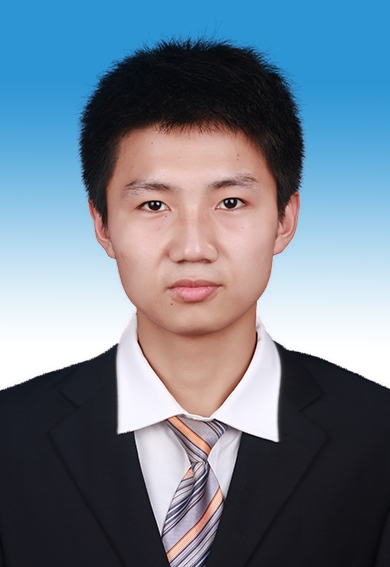
\includegraphics[width=0.88in]{wtx.jpg}} & \scshape{Tianxiong Wu} & \pbar{Java}{0.75} \\
		& \email{wutianxiong626@gmail.com} & \pbar{Scala}{0.5} \\
		& \phone{(+86) 132-8109-5873} & \pbar{Linux}{0.7} \\
		& \linkedin[Tianxiong Wu]{http://www.linkedin.com/in/tianxiong-wu-5156ba103/} & \pbar{Hadoop}{0.5} \\
		& \github[github.com/wtx626]{https://github.com/wtx626} & \pbar{Spark}{0.5}
	\end{tabu}
}
 
\section{\faGraduationCap\  \textbf{教育背景}}
\datedsubsection{\textbf{中南财经政法大学}, 武汉}{2012 -- 2016}
\textit{工学学士}\ 计算机科学与技术
\datedsubsection{\textbf{四川大学}, 成都}{2016 -- 至今}
\textit{在读硕士研究生}\ 计算机技术 

\section{\faHeartO\ \textbf{所获证书}}
\begin{itemize}
\item 四六级证书
\item 软件设计师证书(中级)
\item 软件著作权
\item 优秀硕士研究生证书
\end{itemize}

\section{\faUsers\ \textbf{本科项目经历}}
\datedsubsection{\textbf{中南财经政法大学教务部官方安卓版APP的设计与开发} }{2014.2 -- 2014.6}
APP名称:掌上中南大,于2014年6月上线,用户量达7000。主要功能包括查看课表、成绩查询、空教室查询及一键评教。

\datedsubsection{\textbf{2015年度全国大学生创新训练项目并获国家级重点立项}}{2015.5 -- 2015.12}
项目为《可定制化的心理服务系统》,项目创意来源于当前大学生面对心理问题不敢于去心理咨询室寻求帮助。主要功能包括心理测试、心理美文、在线预约及匿名聊天。

\datedsubsection{\textbf{新加坡国立大学暑期实习}}{2015.7 -- 2015.8}
在NUS计算机学院选修了《计算机思维与技术》、《移动应用程序开发》。通过这两门课程的学习,我深入了解了《算法导论》的相关知识,以及安卓的游戏开发等内容。

\section{\faUsers\ \textbf{硕士研究经历}}
\datedsubsection{\textbf{研究方向}}{}
主要从事基于深度学习的RGB-D人脸识别领域的相关研究,特别关注RGB和Depth之间的异质人脸比对以及如何提升Depth图像的精度。
\datedsubsection{\textbf{公开发表论文(EI检索)}}{}
Liu, Han, et al. "Matching Depth to RGB for Boosting Face Verification." Chinese Conference on Biometric Recognition. Springer, Cham, 2017.

%\section{\faCogs\ \textbf{IT 技能}}
% increase linespacing [parsep=0.5ex]
%\begin{itemize}[parsep=0.5ex]
 % \item 深度学习框架: Caffe, Tensorflow
 % \item 平台: Linux
 % \item 开发:  Web,Android
%\end{itemize}
\section{\faInfo\ 其他}
% increase linespacing [parsep=0.5ex]
\begin{itemize}[parsep=0.5ex]
	\item 技术博客: http://wutianxiong.top
	\item GitHub: https://github.com/wtx626
	\item 语言: 英语 - 熟练
\end{itemize}
\end{document}
